% Template for PLoS
% Version 3.5 March 2018
%
% % % % % % % % % % % % % % % % % % % % % %
%
% -- IMPORTANT NOTE
%
% This template contains comments intended 
% to minimize problems and delays during our production 
% process. Please follow the template instructions
% whenever possible.
%
% % % % % % % % % % % % % % % % % % % % % % % 
%
% Once your paper is accepted for publication, 
% PLEASE REMOVE ALL TRACKED CHANGES in this file 
% and leave only the final text of your manuscript. 
% PLOS recommends the use of latexdiff to track changes during review, as this will help to maintain a clean tex file.
% Visit https://www.ctan.org/pkg/latexdiff?lang=en for info or contact us at latex@plos.org.
%
%
% There are no restrictions on package use within the LaTeX files except that 
% no packages listed in the template may be deleted.
%
% Please do not include colors or graphics in the text.
%
% The manuscript LaTeX source should be contained within a single file (do not use \input, \externaldocument, or similar commands).
%
% % % % % % % % % % % % % % % % % % % % % % %
%
% -- FIGURES AND TABLES
%
% Please include tables/figure captions directly after the paragraph where they are first cited in the text.
%
% DO NOT INCLUDE GRAPHICS IN YOUR MANUSCRIPT
% - Figures should be uploaded separately from your manuscript file. 
% - Figures generated using LaTeX should be extracted and removed from the PDF before submission. 
% - Figures containing multiple panels/subfigures must be combined into one image file before submission.
% For figure citations, please use "Fig" instead of "Figure".
% See http://journals.plos.org/plosone/s/figures for PLOS figure guidelines.
%
% Tables should be cell-based and may not contain:
% - spacing/line breaks within cells to alter layout or alignment
% - do not nest tabular environments (no tabular environments within tabular environments)
% - no graphics or colored text (cell background color/shading OK)
% See http://journals.plos.org/plosone/s/tables for table guidelines.
%
% For tables that exceed the width of the text column, use the adjustwidth environment as illustrated in the example table in text below.
%
% % % % % % % % % % % % % % % % % % % % % % % %
%
% -- EQUATIONS, MATH SYMBOLS, SUBSCRIPTS, AND SUPERSCRIPTS
%
% IMPORTANT
% Below are a few tips to help format your equations and other special characters according to our specifications. For more tips to help reduce the possibility of formatting errors during conversion, please see our LaTeX guidelines at http://journals.plos.org/plosone/s/latex
%
% For inline equations, please be sure to include all portions of an equation in the math environment.  For example, x$^2$ is incorrect; this should be formatted as $x^2$ (or $\mathrm{x}^2$ if the romanized font is desired).
%
% Do not include text that is not math in the math environment. For example, CO2 should be written as CO\textsubscript{2} instead of CO$_2$.
%
% Please add line breaks to long display equations when possible in order to fit size of the column. 
%
% For inline equations, please do not include punctuation (commas, etc) within the math environment unless this is part of the equation.
%
% When adding superscript or subscripts outside of brackets/braces, please group using {}.  For example, change "[U(D,E,\gamma)]^2" to "{[U(D,E,\gamma)]}^2". 
%
% Do not use \cal for caligraphic font.  Instead, use \mathcal{}
%
% % % % % % % % % % % % % % % % % % % % % % % % 
%
% Please contact latex@plos.org with any questions.
%
% % % % % % % % % % % % % % % % % % % % % % % %

\documentclass[10pt,letterpaper]{article}
\usepackage[top=0.85in,left=1.5in,footskip=0.75in]{geometry}
%\usepackage[top=0.85in,left=2.75in,footskip=0.75in]{geometry}
% amsmath and amssymb packages, useful for mathematical formulas and symbols
\usepackage{amsmath,amssymb}

\usepackage{float}

% Use adjustwidth environment to exceed column width (see example table in text)
\usepackage{changepage}

% Use Unicode characters when possible
\usepackage[utf8x]{inputenc}

% textcomp package and marvosym package for additional characters
\usepackage{textcomp,marvosym}

% cite package, to clean up citations in the main text. Do not remove.
\usepackage{cite}

% Use nameref to cite supporting information files (see Supporting Information section for more info)
\usepackage{nameref,hyperref}

% line numbers
\usepackage[right]{lineno}

% ligatures disabled
\usepackage{microtype}
\DisableLigatures[f]{encoding = *, family = * }

% color can be used to apply background shading to table cells only
\usepackage[table]{xcolor}

% array package and thick rules for tables
\usepackage{array}

% for inserting code lines
\usepackage{listings}

\usepackage{adjustbox}
\usepackage{makecell}
% create "+" rule type for thick vertical lines
\newcolumntype{+}{!{\vrule width 2pt}}

% create \thickcline for thick horizontal lines of variable length
\newlength\savedwidth
\newcommand\thickcline[1]{%
  \noalign{\global\savedwidth\arrayrulewidth\global\arrayrulewidth 2pt}%
  \cline{#1}%
  \noalign{\vskip\arrayrulewidth}%
  \noalign{\global\arrayrulewidth\savedwidth}%
}

% \thickhline command for thick horizontal lines that span the table
\newcommand\thickhline{\noalign{\global\savedwidth\arrayrulewidth\global\arrayrulewidth 2pt}%
\hline
\noalign{\global\arrayrulewidth\savedwidth}}


% Remove comment for double spacing
%\usepackage{setspace} 
%\doublespacing

% Text layout
\raggedright
\setlength{\parindent}{0.5cm}
\textwidth 5.25in 
\textheight 8.75in

% Bold the 'Figure #' in the caption and separate it from the title/caption with a period
% Captions will be left justified
\usepackage[aboveskip=1pt,labelfont=bf,labelsep=period,justification=raggedright,singlelinecheck=off]{caption}
\renewcommand{\figurename}{Fig}

% Use the PLoS provided BiBTeX style
\bibliographystyle{plos2015}

% Remove brackets from numbering in List of References
\makeatletter
\renewcommand{\@biblabel}[1]{\quad#1.}
\makeatother



% Header and Footer with logo
%\epstopdfsetup{outdir=./}
\usepackage{lastpage,fancyhdr,graphicx}
\usepackage{epstopdf}
%\pagestyle{myheadings}
\pagestyle{fancy}
\fancyhf{}
\setlength{\headheight}{27.023pt}
%\lhead{\includegraphics[width=2.0in]{PLOS-submission.eps}}
\rfoot{\thepage/\pageref{LastPage}}
\renewcommand{\headrulewidth}{0pt}
\renewcommand{\footrule}{\hrule height 2pt \vspace{2mm}}
\fancyheadoffset[L]{2.25in}
\fancyfootoffset[L]{2.25in}
\lfoot{\today}

%% Include all macros below

\newcommand{\lorem}{{\bf LOREM}}
\newcommand{\ipsum}{{\bf IPSUM}}

%% END MACROS SECTION


\begin{document}
\vspace*{0.2in}

% Title must be 250 characters or less.
%\begin{flushleft}
\centerline{\Large{Machine Learning partie 1}}%{\Large
%\textbf\newline{Machine Learning partie 1} % Please use "sentence case" for title and headings (capitalize only the first word in a title (or heading), the first word in a subtitle (or subheading), and any proper nouns).
\vspace{10mm}
% Insert author names, affiliations and corresponding author email (do not include titles, positions, or degrees).

HEPIA Laroche David\textsuperscript{}

%\end{flushleft}
% Please keep the abstract below 300 words
\section*{Objectif}
Ce projet a pour but de faire pratiquer les méthodologies caractéristiques de l’approche "Data
Science" pour la classification de données. Il se déroulera en trois parties spécifiques associées
aux modèles suivants :
\\
1. modèles de base vus au cours ;
\\
2. ensembles ;
\\
3. réseaux convolutifs.


% Please keep the Author Summary between 150 and 200 words
% Use first person. PLOS ONE authors please skip this step. 
% Author Summary not valid for PLOS ONE submissions.   
\section*{Fonctionnement du script}

\hspace{\parindent} 1. L’exécution du script prend en paramètres optionnels les données à traiter wisc pour \path{wisconsin.dat} et dj pour \path{dow_jones_index.data}, pour les données à choix.\\
2. Il prend aussi les méthode de classification PPV pour le plus proche voisin, AD pour les arbres de décision, PMC pour le perceptron multi-couches et finalement SVM pour la machine à vecteurs de support.\\
3. Le script va donc calculer pour chaque ensemble de données et de classificateurs indiqués avec ses paramètres (définis en durs dans le programme pour des raisons de praticité) puis produire le fichier .csv correspondant.\\
\vspace{1mm}
Ceci permet de comparer les résultats des différents modèles mais aussi quels paramètres influencent le mieux leur taux de classification (TCC).\\
\vspace{1mm}
Exemple de commande :
\begin{lstlisting}[language=bash]
  $ python3 dj wisc PMC AD
\end{lstlisting}

Produit les 4 fichier: \path{output/dj_pmc.csv}, \path{output/dj_ad.csv}, \path{output/wisc_pmc.csv}, \path{output/wisc_ad.csv} contenant les résultats de wisconsin et du dow jones pour les méthodes du perceptron et des arbres de décision.




% Use "Eq" instead of "Equation" for equation citations.
\section*{Choix des données}
J’ai choisi les données de la bourse \verb!dow_jones_index.data!. Presque tous les attributs sont continus. Afin de travailler avec des classificateurs, la classe à prédire a été définie à partir de l’attribut \verb!percent_return_next_dividend!. Ainsi une valeur inférieure à 1 indique une perte et donc appartenant à la classe 0 si elle est supérieure à 1 ceci indique un gain et donc appartenant à la classe 1.
Les données manquantes ont été comblées avec la valeur moyenne des exemples. Finalement tous les attributs continus ont été normalisés.

\section*{Mesure des performances}
\subsection*{Temps de calcul}

Les temps d’entraînement par modèle sont plutôt négligeables.
Par ailleurs, plus un estimateur possède de paramètres, plus il sera coûteux de trouver le meilleur ajustement, car cela implique de calculer un modèle supplémentaire pour chaque combinaison de paramètres. Il est donc judicieux de les limiter et de les choisir de manière intelligente.

\begin{table}[H]
  \centering
  \caption{Temps de Calcul sur les données wisconsin.dat}
  %\label{my-label}
  \begin{adjustbox}{width=\textwidth}
\begin{tabular}{lllll}
\hline
Classificateur & \thead{Nombre de \\modèles entraînés} &
\thead{Temps médian pour \\l’entraînement d’un modèle [msec]} &
Temps total [secondes]
\\ \thickhline
AD & \hspace{5mm}32076 & \hspace{20mm}1.2 & \hspace{10mm}247  \\ \hline
PPV & \hspace{5mm}50 & \hspace{20mm}0.9 & \hspace{10mm}5.11\\ \hline
PMC & \hspace{5mm}432 & \hspace{20mm}731 & \hspace{10mm}774\\ \hline
\end{tabular}
\end{adjustbox}
\end{table}

\begin{table}[h]
  \centering
  \caption{Temps de Calcul sur les données \protect\path{dow_jones_index.data}}
  %\label{my-label}
  \begin{adjustbox}{width=\textwidth}
\begin{tabular}{lllll}
\hline
Classificateur & \thead{Nombre de \\modèles entraînés} &
\thead{Temps médian pour \\l’entraînement d’un modèle [msec]} &
Temps total [secondes]
\\ \thickhline
AD & \hspace{5mm}32076 & \hspace{20mm}3.2 & \hspace{10mm}525  \\ \hline
PPV & \hspace{5mm}50 & \hspace{20mm}0.9 & \hspace{10mm}5.8\\ \hline
PMC & \hspace{5mm}432 & \hspace{20mm}837 & \hspace{10mm}868\\ \hline
\end{tabular}
\end{adjustbox}
\end{table}

Nous pouvons observer que l’AD et le PPV sont peu coûteux en calculs (temps médian par modèle) contrairement au PMC  qui est assez lourd en comparaison.


\subsection*{Validation croisée}
Le nombre de sous échantillons que l’on choisis pour la validation croisée augmente grandement les temps de calculs car nous multiplions le nombre de résultats par le nombre d’échantillons à entraîner. J’ai donc commencé avec une division en 3 sous-échantillons afin de trouver les paramètres et ai terminé avec 10 segments comme demandé pour obtenir des résultats plus réalistes en les moyennant.
\newpage
\subsection*{Taux de classification}
Voici le meilleur taux de classification correct (TCC) moyen en calculant la moyenne des résultats obtenus de la validation croisée avec dix sous-échantillons (méthode : k-fold cross-validation).

\begin{table}[h]
  \centering
  \caption{Meilleur TCC par Classificateur sur les données wisconsin.dat}
  %\label{my-label}
  %\begin{adjustbox}{width=\textwidth}
\begin{tabular}{lll}
\hline
Classificateur & TCC moyen test 
 & TCC moyen entraînement
\\ \thickhline
AD & \hspace{5mm}0.88 & \hspace{20mm}0.88
 \\ \hline
PPV & \hspace{5mm}0.97 & \hspace{20mm}0.98 \\ \hline
PMC & \hspace{5mm}0.97 & \hspace{20mm}0.98\\ \hline
\end{tabular}
%\end{adjustbox}
\end{table}

\begin{table}[h]
  \centering
  \caption{Meilleur TCC par Classificateur sur les données  \protect\path{dow_jones_index.data}}
  %\label{my-label}
  %\begin{adjustbox}{width=\textwidth}
\begin{tabular}{lll}
\hline
Classificateur & TCC moyen test 
 & TCC moyen entraînement
\\ \thickhline
AD & \hspace{5mm}0.92 & \hspace{20mm}0.94
 \\ \hline
PPV & \hspace{5mm}0.88 & \hspace{20mm}1 \\ \hline
PMC & \hspace{5mm}0.97 & \hspace{20mm}0.98\\ \hline
\end{tabular}
%\end{adjustbox}
\end{table}
Les performances entre classificateurs sont assez proches. 
Les TCC des sets d’entraînement sont légèrement supérieurs aux TCC des tests ce qui est attendu car le modèle est entraîné avec le set d’entraînement par définition. Mais la différence de valeurs entre TCC test et TCC entraînement n’est pas assez grande pour indiquer avec assurance un overfitting. 
Seule la valeur du TCC au-delà de 95 \% indiquerai une performance trop grande et donc un overfitting sur nos données malgré l’utilisation de la validation croisée.

\subsection*{Plus Proche Voisin}
Paramètres modifiés:\\
1. Nombre de vosins pour la requête [\verb!n_neighbours!]: nombre impair de 1 à 50\\
2. Poids pour la requête: [uniform, distance]\\
\vspace{1mm}
Ce classificateur ne possédant que deux paramètres nous intéressant dont un binaire nous pouvons représenter les résultats sur un graphe.

\begin{figure}[H]
\centering
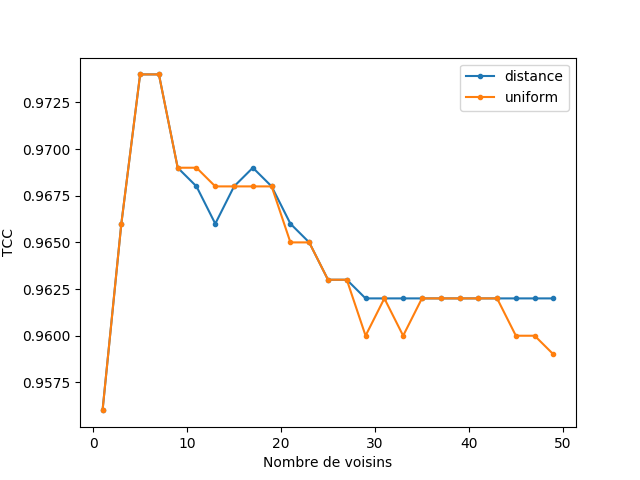
\includegraphics[scale=0.65]{wisc_ppv.png}
\caption{Plot on wisconsin.data}
\end{figure}
Nous avons un maximum à 5 et 7 voisins, ensuite l’augmentation de ce nombre n’améliore pas la performance. Les dents de scies sur le même nombre de voisins est causé par le mode de détermination de la classe (par distance ou par majorité). Avec ces données, le changement des paramètres influence peu la performance (différence de 1,8 point entre le maximum et le minimum).

\begin{figure}[H]
\centering
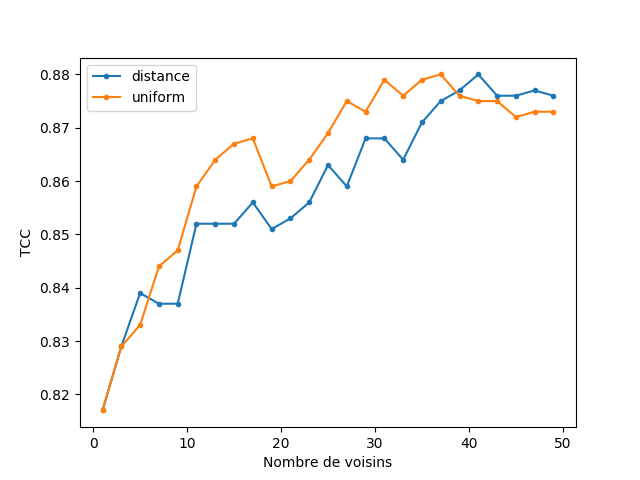
\includegraphics[scale=0.65]{dj_ppv.png}
\caption{Plot on \protect\path{dow_jones_index.data}}
\end{figure}

Cette courbe fait penser à la fonction logarithme, le TCC s’améliore avec l’augmentation de [\verb!n_neighbours!] pour définir la classe mais devient de plus en plus plate.

\subsection*{Arbre de Décision}
Paramètres modifiés:\\
1. Profondeur maximale (\verb!max_depth!) : 1 à 99\\
2. Nombre d’exemples minimum par feuille (\verb!min_samples_leaf!) : 2 à 20\\
3. Nombre minimal pour le découpage d’une node (\verb!min_samples_split!) : 2 à 20\\

\vspace{2mm}
Le découpage d’une node se fait avec le meilleur gini par défaut.


\begin{table}[h]
  {\centering
  \caption{Meilleurs scores sur wisconsin.dat}
  \label{table:scores_wisc}
  \begin{adjustbox}{width=\textwidth}
\begin{tabular}{lllllll}
\hline
\thead{TCC \\Test\\ Moyen} & STD & \thead{TCC\\ Train \\Moyen} & \thead{Fit \\Time\\ Moyen} & Max Depth & \thead{Min \\Samples \\Leaf} & \thead{Min \\Samples \\Split}
\\ \thickhline

0.875 & 0.03 & \hspace{5mm}0.88 & \hspace{5mm}0.002 & \hspace{5mm}1 & \hspace{5mm}2 &\hspace{5mm}2 \\ \hline
0.875 & 0.03 & \hspace{5mm}0.88 & \hspace{5mm}0.002 & \hspace{5mm}99 & \hspace{5mm}19 &\hspace{5mm}19 \\ \hline
\end{tabular}
\end{adjustbox}}
\footnotesize{Par soucis de représentation j’ai omis les 100 modèles (ou lignes) possédant le même TCC Test Moyen (0.875), [\verb!max_depth!] augmentant de 1 à chaque ligne
}
\end{table}
Nous pouvons observer (ref. Table \ref{table:scores_wisc}) que [\verb!max_depth!] n’influence pas le TCC test moyen (\verb!mean_test_score!) pour une certaine combinaison des paramètres [\verb!min_samples_leaf!] et [\verb!min_samples_split!].\\
\vspace{2mm}
Il est tout a fait possible que certains paramètres comme [\verb!min_samples_leaf!] arrêtent la croissance de l’arbre avant d’arriver à la profondeur maximale, ainsi [\verb!max_depth!] ne produit aucune amélioration du TCC à partir d’un certain seuil. Nous pouvons avoir le même phénomène avec le nombre d’exemple minimal pour découper une node. Ces paramètres s’influence donc entre eux mais sont utiles pour se prémunir de l’overfitting, le pire des cas étant d’avoir une feuille pour chaque exemple.

\begin{table}[h]
  {\centering
  \caption{Meilleurs scores sur \protect\path{dow_jones_index.data}}
  \label{table:scores_dj}
  \begin{adjustbox}{width=\textwidth}
\begin{tabular}{lllllll}
\hline
\thead{TCC \\Test\\ Moyen} & STD & \thead{TCC\\ Train \\Moyen} & \thead{Fit \\Time\\ Moyen} & Max Depth & \thead{Min \\Samples \\Leaf} & \thead{Min \\Samples \\Split}
\\ \thickhline
0.923 & 0.09 & \hspace{5mm}0.94 & \hspace{5mm}0.002 & \hspace{5mm}3 & \hspace{5mm}2 &\hspace{5mm}7 \\ \hline
0.923 & 0.09 & \hspace{5mm}0.94 & \hspace{5mm}0.002 & \hspace{5mm}3 & \hspace{5mm}19 &\hspace{5mm}19 \\ \hline
\end{tabular}
\end{adjustbox}}
\footnotesize{Par soucis de représentation j’ai omis les 170 modèles (ou lignes) possédant le même TCC Test Moyen (0.923), tous ces modèles possèdent le même [\verb!max_depth!] de 3.}
\end{table}

Sur ces données Table \ref{table:scores_dj} c’est la profondeur de l’arbre qui influence le plus les résultats, la profondeur restant à 3 malgré le changement des deux derniers paramètres pour les meilleurs TCC Test Moyen. On peut supposer que peu d’attributs suffisent à trouver la meilleure prédiction, le reste étant du bruit, il serait utile des les négliger dans nos modèles.

\newpage


\subsection*{Perceptron Multi Couches}
Paramètres modifiés:\\
    1. Fonction d’activation (activation) : Identité, Tangente hyperbolique (tanh), Logistique, Unité de rectification linéaire (relu)\\
    2. Alpha : 0.1, 1, 10\\
    3. couches cachées et nombre de neurones y figurant (\verb!hidden_layer_sizes!) : (5, 50), (5, 100), (10, 50), (10,100)\\
    4. Taux d’apprentissage (\verb!learning_rate!) : constant, invscaling, adaptif\\
    5.  solveur : lbfgs, sgd, adam\\


\begin{figure}[H]
\centering
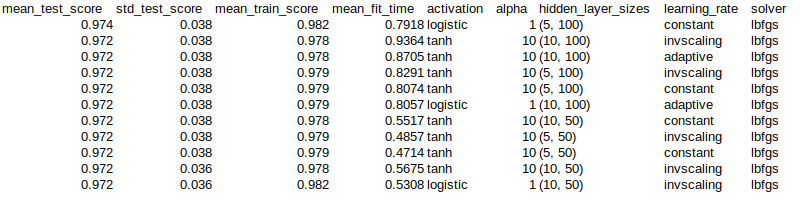
\includegraphics[scale=0.65]{wisc_pmc_1.png}
\caption{Meilleurs scores sur wisconsin.dat}
\end{figure}

Pour le PMC nous obtenons les meilleurs résultats avec un alpha de 1 ou 10 et la fonction d’activation tangente hyperbolique le plus souvent et lbfgs comme solveur.
Dans notre cas, nombre de de couches cachées et le nombres de neurones y figurant influencent peu les résultats.
Je suppose que le alpha de 0.1 systématiquement plus mauvais dans notre cas est causé par la tendance à rester dans des minimas locaux moins bons lors de la descente de gradient.
\newpage
Le TCC minimum obtenu est de 0.439 ce qui est mauvais. Nous pouvons déduire que la configuration des paramètres est d’autant plus important pour ce classificateur. Cependant, à part les trois paramètres cités avant, il est difficile de déterminer quelle est l’influence des autres paramètres car c’est sans doute leur combinaison qui explique cette variation de résultats.

Variation que nous pouvons observer si nous classons les modèles par ordre de TCC décroissant.

\begin{figure}[H]
\centering
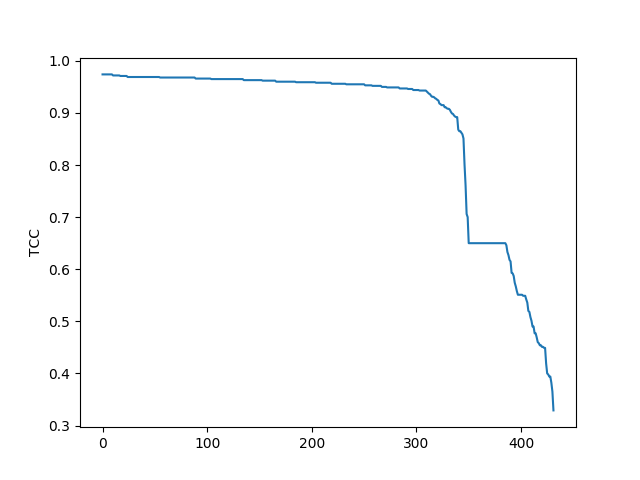
\includegraphics[scale=0.65]{wisc_pmc_2.png}
\caption{Décroissance du TCC sur wisconsin.data}
\end{figure}

Nous pouvons remarquer un saut de 0,9 à 0,65 environ de TCC, en étudiant les données, la combinaison des autres paramètres avec la fonction logistique donne systématiquement des résultats moins bon, ainsi qu’une combinaison entre certains paramètres et le solveur invscaling.


\begin{figure}[H]
\centering
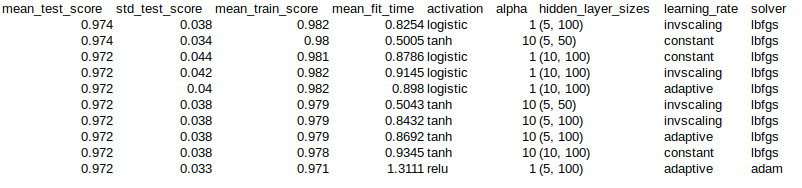
\includegraphics[scale=0.65]{dj_pmc_1.png}
\caption{Meilleurs scores sur \protect\path{dow_jones_index.data}}
\end{figure}

Il intéressant de relever la similarité des scores et des meilleurs paramètres malgré deux ensembles de données très différents.
On observe le même phénomène si l’on classe les modèles par TCC.

\begin{figure}[H]
\centering
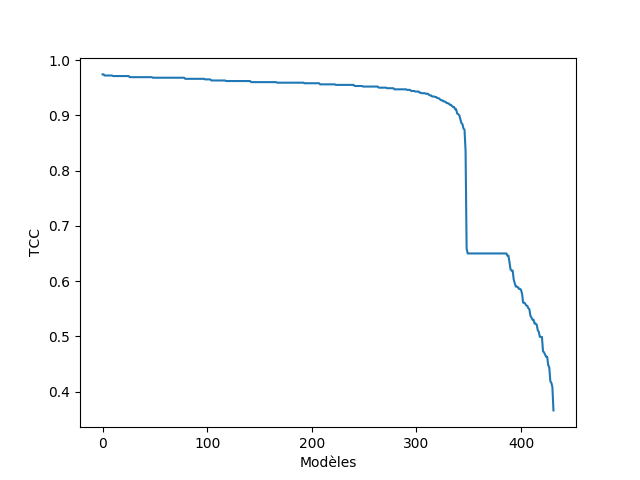
\includegraphics[scale=0.65]{dj_pmc_2.png}
\caption{Décroissance du TCC sur\protect\path{dow_jones_index.data}}
\end{figure}

% Results and Discussion can be combined.
\section*{Conclusion}

Scikitlearn fournit beaucoup d’outils pour améliorer ses modèles de classification ou de régression. Cependant il n’est pas toujours évident de comprendre l’influence des paramètres utilisés, une idée serait d’utiliser une régression sur ces données (donc du machine learning sur du machine learning...) afin de déterminer les paramètres les plus influents en comparant leurs poids. Il serait aussi judicieux d’étudier le domaine de la statistique qui possède des liens forts avec le machine learning, mais le champ est vaste...

% Either type in your references using
% \begin{thebibliography}{}
% \bibitem{}
% Text
% \end{thebibliography}
%
% or
%
% Compile your BiBTeX database using our plos2015.bst
% style file and paste the contents of your .bbl file
% here. See http://journals.plos.org/plosone/s/latex for 
% step-by-step instructions.
% 
\vspace{15mm}
\begin{thebibliography}{10}

\bibitem{bib1}
\url{https://scikit-learn.org}
%Conant GC, Wolfe KH.
%\newblock {{T}urning a hobby into a job: how duplicated genes find new
%  functions}.
%\newblock Nat Rev Genet. 2008 Dec;9(12):938--950.

\end{thebibliography}

\end{document}
